\documentclass[crop,class=article]{standalone}
%----------------------------Preamble-------------------------------%
\usepackage{tikz}                       % Drawing/graphing tools.
\usetikzlibrary{arrows.meta}            % Latex and Stealth arrows.
%--------------------------Main Document----------------------------%
\begin{document}
    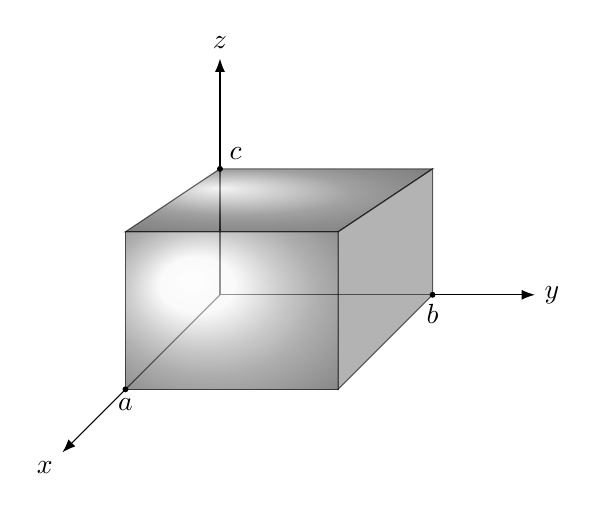
\begin{tikzpicture}[%
        line width=0.4pt,
        line cap = round,
        >={Latex}
    ]
        \draw[->] (0,0) -- (4,0) node[right] {$y$};
        \draw[->] (0,0) -- (0,3) node[above] {$z$};
        \draw[->] (0,0) -- (-2,-2) node[below left] {$x$};
        \draw[ball color=gray!10!white,opacity=0.6]
            (-1.2,-1.2) to (1.5,-1.2) to (1.5,0.8)
                        to (-1.2,0.8) to cycle;
        \draw[ball color = gray!90!white,opacity=0.6]
            (-1.2,0.8) to (0,1.6) to (2.7,1.6)
                       to (1.5,0.8) to cycle;
        \draw[fill=gray,opacity=0.6]
            (1.5,0.8) to (2.7,1.6) to (2.7,0)
                      to (1.5,-1.2) to cycle;
        \draw[fill=black] (-1.2,-1.2) circle (0.03)
            node [below] {$a$};
        \draw[fill=black] (0,1.6) circle (0.03)
            node [above right] {$c$};
        \draw[fill=black] (2.7,0) circle (0.03)
            node [below] {$b$};
    \end{tikzpicture}
\end{document}